\newcommand{\btb}{^{(t)}}
\newcommand{\btprevb}{^{(t-1)}}
\newcommand{\btnextb}{^{(t+1)}}


\renewcommand{\vec}[1]{\mathbf{#1}} % my vector definition
\newcommand{\eqdef}{=}

\subsection{Self-adaptation in Evolution Strategies}

Evolution strategies and many other evolutionary algorithms for
real-valued optimization usually rely on Gaussian random mutations. That is,
candidate solutions are altered by adding random vectors drawn
according to zero-mean normal distributions.  Adaptation of the
covariance matrices of these random variations during optimization
allows for learning and employing an appropriate metric for the search
process.  It is well known that an automatic adaptation of the
mutation distribution drastically improves the search performance on
non-separable or badly scaled objective functions
\cite{Rechenberg:94,Schwefel:95,hansen:01,beyer:02b,kern:04}.


 The original approaches to the adaptation of the covariance matrix 
add  parameters describing the matrix to the chromosome of each individual and rely
on a ``second-order'' selection process for their choice. This is
termed self-adaptation of strategy parameters in ES. In the following, we
will give a short overview over the different methods, which are
implemented in the library.
%; the syntax of the different operators is
%summarized in Section \ref{classReference:sec:EALib}.

% Whenever it is beneficial for the search process to move along the,
% say, $x_1$ coordinate in a specific proportion to the distance along
% the $x_2$ coordinate, we speak of the need for correlated
% mutations. Several schemes exist that incorporate correlations between
% the variations.
% The most intuitive way is to rotate the matrix of
% variances, as first proposed by Schwefel and described in
% \cite{Baeck:96}. All other methods from the ``derandomized'' approach to 
% self-adaptation in ES include correlated mutations in one way or the
% other. The simplest method to adapt the complete correlation matrix is
% difficult, since it cannot be guaranteed that the resulting system
% will remain orthogonal and allow mutations in any direction 
% (for this reason the number of vectors in the generating set 
% approach in Section \ref{ss:GenSet} have to be consistently 
% larger than $n$ (dimension of the search space).
%Besides including correlated mutations along the axes, there is 
%another approach to improve evolution strategies.
The ``derandomized'' adaptation put forward by Ostermeier
\cite{Ostermeier:92,Ostermeier:94} aims at a more direct adaptation of
the strategy parameters. In the standard evolution strategy the
adaptation has to overcome the stochastic fluctuations which are
introduced by the fact that even distributions with small variances
can produce large values and vice versa. This source of ``noise'' in
the adaptation process is circumvented by using the actual
step-length, that is, the realization of the random number $z$ for the
adaptation. In addition, to the derandomization the idea of an
``evolution path'' is inherent in all of these approaches. The
principle is very similar to a momentum term in standard gradient
descent approaches. The adaptation does not just rely on the step
which is chosen in the current generation but also on selected steps
in previous generation.

% The following short overview introduces the
% different strategies. More detailed information can be found in 
% \cite{Baeck:96,Rechenberg:94,Schwefel:95} for Sections 
% \ref{ss:standard} and \ref{ss:rotate}, in 
% \cite{Hansen:98,Hansen:95,Ostermeier:94} for Sections \ref{ss:GenSet}
% and \ref{ss:IndDir}, and in \cite{Hansen:98,Hansen:96} for Section
% \ref{ss:CMA}.

\subsubsection{Standard adaptation}
\label{ss:standard}
In the standard evolution strategy, the mutation of the objective
variables $\vec{x}$ is carried out by adding a $N(0,\sigma_i^2)$ 
distributed random number $z_i$ to each component of $x_i$. The
``step-sizes'' $\sigma_i$ are also subject to mutations
(log-normal distributed) both for each component separately
(parameterized by $\tau$) and overall (parameterized by $\tau'$).
Thus, the individual consists of both the objective and the step-size 
vector. 
\begin{eqnarray}
\sigma_i\btb & = & \sigma_i\btprevb \exp( \tau' \, z) \; \exp( \tau \,z_i)\\
\vec{x}\btb & = & \vec{x}\btprevb + \vec{\tilde z}\\
z_i, z & \sim & N(0,1)\\
\vec{\tilde z}& \sim & N\left(\vec{0}, \left({\vec{{\tilde \sigma}}\btb}\right)^{2}\right).
\end{eqnarray}
This is the
standard evolution strategy according to \cite{Baeck:96,Schwefel:95}.
The version put forward by \cite{Rechenberg:94} is different,
particularly with respect to the changes of the ``step-size'':
\begin{eqnarray}
\sigma_i\btb & = & \sigma_i\btprevb \,\xi,\\
\vec{x}\btb & = & \vec{x}\btprevb + \vec{\sigma}\cdot \vec{z}\\
z_i & \sim & N(0,1/n)
\end{eqnarray}
$\xi$ has the value $1.5$ with probability $\xi_{prob}$ and 
the value $1/1.5$ with probability $(1-\xi_{prob})$. In the standard
method in \cite{Rechenberg:94}, $\xi_{prob} = 0.5$.
$n$ is the dimension of the objective vector. The 
variance $1/n$ guarantees that the length $||z||$ is one on average
for large $n$.

\subsubsection{Rotation matrix adaptation}
\label{ss:rotate}
Instead of adapting the complete correlation matrix $\vec{C}$ of the
$n$-dimensional normal distribution (eq. \ref{fullCorr}), 
it is sufficient to rotate the diagonal matrix 
$\vec{C'}=diag(\sigma_1,\ldots,\sigma_n)$ using $n(n-1)/2$ rotation angles.
\begin{equation}
\label{fullCorr}
p(\vec{z}) = \frac{1}{(2\pi)^{n/2} \det \vec{C}}
\exp\left(-\frac{1}{2}\vec{z}^T\,\vec{C}^{-1}\,\vec{z}\right).
\end{equation}
The rotations can be written as follows using the rotation matrices
$\vec{R}(\alpha_{ij})$:
\begin{eqnarray}
\vec{R}(\alpha_{ij}) & = & \left( \begin{array}{ccccc}
1 & 0 & \cdots & \cdots &  0 \\
0 & 1 & \cdots & \cdots &  0 \\
\cdots & \cos \alpha_{ij} & \cdots & - \sin \alpha_{ij} & \cdots\\
\cdots & \cdots & \cdots & \cdots &  \cdots \\
\cdots & \sin \alpha_{ij} & \cdots & \cos \alpha_{ij} & \cdots\\
\cdots & \cdots & \cdots & \cdots &  \cdots \\
0 & \cdots & \cdots & 0 & 1
\end{array}\right)\\
\vec{{\tilde \sigma}} & = & \left( \prod^{n-1}_{i=1}\prod_{j=i+1}^{n}
\vec{R}(\alpha_{ij}) \right) \cdot \vec{\sigma}
\end{eqnarray}
The trigonometric functions occur in $\vec{R}(\alpha_{ij})$ at the
positions $(row, column) =(i,i), (i,j), (j,i), (j,j).$
Mutation of the $n$ step sizes $\vec{\sigma}$ and the mutation angles
is carried out like in the standard algorithm
\begin{eqnarray}
\sigma_i\btb & = & \sigma_i\btprevb \exp( \tau' \, z) \; \exp( \tau \,z_i)\\
\alpha_{ij}\btb & = & \alpha_{ij}\btprevb + \beta \,z^{\alpha}_{ij}\\
\vec{x}\btb & = & \vec{x}\btprevb + \vec{\tilde z}\\
z_i, z, z^{\alpha}_{ij} & \sim & N(0,1)\\
\vec{\tilde z}& \sim & N(\vec{0}, \vec{{\tilde \sigma}}\btb).
\end{eqnarray}
The values of $\alpha_{ij}$ are confined to the interval $[-\pi,\pi]$
and a lower bound can be defined for the $\sigma_i$ (in the function
this is determined by the values of {\em toggle} and $\epsilon$).
The standard setting of the parameters is shown in Table 
\ref{RotateParams}, two
versions of the operator {\sffamily\bfseries\small mutateRotate}
exist, one which includes the standard values and one where all
variables have to be defined explicitly. 


% The composition of
% the chromosome is shown in Figure \ref{StdBelegung} (a).
\begin{table}
\centerline{
\begin{tabular}{c|c|l}
\hline
Parameter & Standard Value & Comment \\
\hline
$\tau'$ & $1/\sqrt{2n}$  & heuristic value \\
$\tau$ & $1/\sqrt{2\sqrt{n}}$ & heuristic value \\
$\beta$ & $0.0873$  & heuristic value \\
{\em toggle} & FALSE & enforce lower bound \\
$\epsilon$ &   & lower bound for $\sigma$ \\
\hline
\end{tabular}}
\hfill\\
\caption[T1]{\label{RotateParams}Parameters for the rotation angle
  adaptation and their standard values; $n$ is the dimension of the
  objective vector $\vec{x}$.} 
\end{table}
% \begin{figure}
% \includegraphics[width=0.7\columnwidth]{esStds.eps}
% \caption{\label{StdBelegung}The position of the various mutation
%   parameters for the different self-adaptation schemes in the chromosome
%   \emph{stddev}. (a) Rotation matrix adaptation, 
%   (b) generating set adaptation, (c) individual step sizes and 
%   one direction adaptation, (d) covariance matrix adaptation.}
% \end{figure}



\subsubsection{The $(\mu_{\vec w},\lambda)$-CMA Evolution Strategy}\label{sec:cma}
%
\paragraph{Basic Principles}
In the CMA-ES \cite{hansen2003rtc,Hansen2006} a parent population of
$\mu$ candidate solutions are maintained, from which $\lambda>\mu$ new
candidate solutions are generated in each iteration. The performances
of these offspring solutions  are determined and the $\mu$
best form the parent population in the next iteration.  In each
iteration, the $k$th offspring $\vec{x}_k\in\mathbbm R^n$ is generated
by multi-variate \emph{Gaussian mutation} and \emph{weighted global
  intermediate recombination}, i.e.,
\[\vec{x}_k=\left<\vec{x}_{\text{parents}}\right>_{\vec w}
+\sigma\vec{z}_k,\] where $\vec{z}_k\sim \text{N}(\vec 0, \vec C)$ and
\[\left<{\vec{x}}_{\text{parents}}\right>_{\vec w} = \sum_{i=1}^\mu w_i
{\vec x}_{\text{$i$th-best-parent}}\] 
(a common chice is $\vec w_i\propto \ln(\mu+1) -
\ln(i)$, $\|\vec w\|_1=1$).
%
The CMA-ES is a variable metric algorithm adapting both the
$n$-dimensional covariance matrix $\vec C$ of the normal mutation
distribution as well as the \emph{global step size } $\sigma\in\mathbbm
R^+$. In the basic algorithm, a low-pass filtered \emph{evolution
  path} $\vec{p}$ of successful directions (i.e., selected steps) is
stored, \[\vec{p} \leftarrow \eta_1\, \vec{p} +
\eta_2\,\left(\left<{\vec{x}}_{\text{new
        parents}}\right>-\left<{\vec{x}}_{\text{old
        parents}}\right>\right),\] and $\vec{C}$ is changed to make
steps in the direction $\vec{p}$ more likely: $\vec{C} \leftarrow
\eta_3\, \vec{C}+ \eta_4\,\vec{p}\vec{p}^T$ (this rank-one update of $\vec C$ is augmented by a
rank-$\mu$ update, see \cite{hansen2003rtc}).
%
The variables $\eta_1,\dots,\eta_4$ denote fixed learning rates and
normalization constants set to default values, see below.  The global
step size $\sigma$ is adapted on a faster timescale.  It is increased
if the selected steps are larger and/or more correlated than expected
and decreased if they are smaller and/or more anticorrelated than
expected.
%
The highly efficient use of information and the fast adaptation of
$\sigma$ and $\vec C$ makes the CMA-ES one of the best direct search
algorithms for real-valued optimization. 

\paragraph{Details}
  In the following, we present the details of
the covariance matrix adaptation ES 
with weighted recombination and rank-$\mu$-update
$(\mu_{\vec w},\lambda)$-CMA-ES) as described in
\cite{hansen2003rtc,Hansen2006}, which is based on 
\cite{Hansen:96,hansen:01}. 

Each individual represents an $n$-dimensional
real-valued object variable vector.  These variables are altered by
two variation operators, intermediate recombination and additive
Gaussian mutation.  The former corresponds to computing the 
(possibly weighted) center of
mass of the $\mu$ individuals in the parent population.  Mutation is
realized by adding a normally distributed random vector with zero
mean.  The complete covariance matrix of the Gaussian
mutation distribution is adapted during evolution to improve the
search strategy.  


The object parameters $\vec{x}_k\btnextb$ of offspring
$k=1,\dots,\lambda$ created in generation $g+1$ are given by
\begin{equation}
\vec{x}_k\btnextb=\left<{\vec{x}}\right>\btb_{\vec w}+\sigma\btb\vec{B}\btb\vec{D}\btb\vec{z}\btb_k \enspace,
\end{equation}
where the $\vec{z}\btb_k\sim {N}(\vec{0},\vec{I})$ are
independent realizations of an $n$-dimensional normally distributed
random vector with zero mean and covariance matrix equal to the
identity matrix $\vec{I}$ and
\begin{equation}
\left<{\vec{x}}\right>\btb_{\vec w}=\sum_{i=1}^\mu
w_i \vec{x}_{i:\lambda}\btb
\end{equation}
is the weighted mean of the selected individuals with
\begin{equation}\label{wnormal:eq}
\sum_{i=1}^\mu w_i = 1
\end{equation}
and $w_i>0$ for $i=1,\dots,\mu$. The index $i:\lambda$
denotes the $i$th best individual. 
%
The covariance matrix $\vec{C}\btb$ of the random vectors
\begin{equation}
\vec{B}\btb\vec{D}\btb\vec{z}\btb_k\sim {N}(\vec{0},\vec{C}\btb)
\end{equation}
is a symmetric positive $n\times n$ matrix with
\begin{equation}
{\vec{C}}\btb=\vec{B}\btb\vec{D}\btb\left(\vec{B}\btb\vec{D}\btb\right)^T\enspace.
\end{equation}
The columns of the orthogonal $n\times n$ matrix $\vec{B}\btb$ are
the normalized eigenvectors of ${\vec{C}}\btb$ and $\vec{D}\btb$
is a $n\times n$ diagonal matrix with the square roots of the
corresponding eigenvalues.  Figure \ref{fig:cma} schematically shows
the transformations of $\vec{z}\btb_k$ by %$\sigma\btb$,
$\vec{B}\btb$ and $\vec{D}\btb$.
                                                                                                                                                                
\begin{figure}
{
  \psfrag{d}[B][B]{\small $\times$}
  \psfrag{a}[B][B]{\small $\vec{z}_l\btnextb$}
  \psfrag{b}[B][B]{\small $\vec{D}\btb\vec{z}_l\btnextb$}
  \psfrag{c}[B][B]{\small $\vec{B}\btb\vec{D}\btb\vec{z}_l\btnextb$}
% \centerline{\epsfig{file=distributionPhd.eps,width=.75\textwidth}}
 \centerline{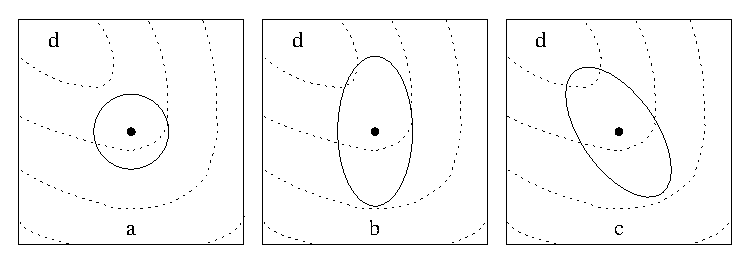
\includegraphics[width=.9\textwidth]{cmascheme.eps}}
}
\caption{\label{fig:cma}   The
  dashed lines schematically visualize an error\,/\,fitness surface
  (landscape) for $\subset{\mathbbm R}^2$, where each line
  represents points of equal fitness and the $\times$ symbol marks the
  optimum. The dot corresponds to the center of mass of the parent
  population and the solid lines indicate the mutation
  \mbox{(hyper-)}\,ellipsoids (i.e., surfaces of equal probability
  density to place an offspring) of the random vectors after the
  different transformations.
%
  Evolution strategies that adapt only one global step size can only
  produce mutation ellipsoids as shown in the left plot. Algorithms
  that adapt $n$ different step sizes, one for each object variable,
  can produce mutation ellipsoids scaled along the coordinate axes
  like the one shown in the center plot.  Only if the complete
  covariance matrix is adapted, arbitrary normal distributions can be
  realized as shown in the right picture.
}
\end{figure}
                                                                                
                                                                                
                                                                                
The strategy parameters, both the matrix ${\vec{C}}\btb$ and the so
called global step-size $\sigma\btb$, are updated online using the
covariance matrix adaptation (CMA) method.  The key idea of the CMA is
to alter the mutation distribution in a deterministic way such that
the probability to reproduce steps in the search space that have led
to the current population is increased.
%
This enables the algorithm to detect correlations between object variables
and to become invariant under orthogonal transformations of the search
space (apart from the initialization). In order to use the information
from previous generations efficiently, the search path of the
population over a number of past generations is taken into account.
                                                                                
In the CMA-ES, rank-based $(\mu,\lambda)$-selection is used for
environmental selection. That is, the $\mu$ best of the $\lambda$
offspring form the next parent population.  After selection, the
strategy parameters are updated:
\begin{align}\label{pathAdapt:eq}
  \vec{p}\btnextb &= (1-c_c)\cdot\vec{p}_c\btb+
\sqrt{c_c(2-c_c)}\frac{\sqrt{\mu_\text{eff}}}{\sigma\btb}
\left(\left<{\vec{x}}\right>\btnextb-\left<{\vec{x}}\right>\btb\right)\enspace,\\
%\end{equation}\vspace{-\topsep}
%\begin{equation}\label{covariance:eq}
\vec{C}\btnextb &= (1-c_{\text{cov}})\cdot {\vec{C}}\btb
  + c_{\text{cov}}\cdot 
\left(\frac{1}{\mu_{\text{cov}}}
\vec{p}\btnextb
  \left(\vec{p}\btnextb \right)^{\text{T}}\right.\nonumber\\
&\left.+\left(1-\frac{1}{\mu_{\text{cov}}}\right)
\sum_{i=1}^\mu
\frac{w_i}{{\sigma\btb}^2}
\left(\vec{x}_{i:\lambda}\btnextb-\left<{\vec{x}}\right>\btb_{\vec w} \right)
\left(\vec{x}_{i:\lambda}\btnextb-\left<{\vec{x}}\right>\btb_{\vec w} \right)^T
\right)
\enspace.\label{covariance:eq}
\end{align}
Herein, $\vec{p}\btnextb\in {\mathbbm R}^n$ is the evolution path---a
weighted sum of the centers of the population over the generations
starting from $\vec{p}^{(0)}\eqdef\vec 0$
(the factor $\sqrt{\mu_\text{eff}}$ compensates for the loss of variance due to
computing the center of mass). The parameter $c_c\in\, ]0,1]$ controls
the time horizon of the adaptation of $\vec{p}$.  The constant
$\sqrt{c_c(2-c_c)}$ normalizes the variance of $\vec{p}$
(viewed as a random variable) as $1^2=(1-c)^2+ (\sqrt{c_c(2-c_c)})^2$.  
The index $i$$:$$\lambda$ is the index of
the offspring having the $i$th best fitness value of all offspring in
the current generation.
The parameter $c_{\text{cov}}\in [0,1[\,$ controls the update of
${\vec{C}}\btb$. The vector
$\vec{p}$ does not only represent the last (adaptive) step of
 the parent population, but a time average over
all previous adaptive steps. The influence of previous steps
decays exponentially, where the decay rate is controlled by $c_{\text{cov}}$.
                                                                                
The first line of the update rule (\ref{covariance:eq}) shifts $\vec{C}\btb$ towards
the $n\times n$ matrix
$\vec{p}\btnextb\left(\vec{p}\btnextb\right)^T$, which has rank 1, making mutation steps
in the direction of $\vec{p}\btnextb$ more likely.  
The second line is the rank-$\mu$-update, which is particularly useful in case
of large populations: the matrix resulting from the sum over all selected
offspring has rank $\min(\mu,n)$.
                                                                                

The adaptation of the global step-size parameter $\sigma$ is done
separately on a faster timescale (a single parameter can be estimated
based on less samples compared to the complete covariance matrix).  We
keep track of a second evolution path $\vec{p}_\sigma$ without the
scaling by $\vec{D}$:
\begin{align}
  \vec{p}\btnextb_\sigma&=(1-c_\sigma)\cdot\vec{p}\btb_\sigma\nonumber\\
  &+\sqrt{c_\sigma(2-c_\sigma)}\cdot\vec{B}\btb {\vec{D}\btb}^{-1} {\vec{B}\btb}^{T}\frac{\sqrt{\mu_\text{eff}}}{\sigma\btb}
\left(\left<{\vec{x}}\right>\btnextb-\left<{\vec{x}}\right>\btb\right)\enspace,\\
\sigma\btnextb&=\sigma\btb\cdot\exp\left(\frac{c_\sigma}{d_\sigma}\left(\frac{\|\vec{p}\btnextb_\sigma\|
    - \hat{\vec{\chi}}_n}{\hat{\vec{\chi}}_n}\right)\right)
\enspace,\label{globalAdapt2:eq}
\end{align}
where $\hat{\vec{\chi}}_n$ is the expected length of a
$n$-dimensional, normally distributed random vector with covariance
matrix $\vec I$. It is approximated by
$\sqrt{n}(1-\frac{1}{4n}+\frac{1}{21n^2}$.  The damping parameter
$d_{sigma}$ decouples the adaptation rate from the strength of the
variation.  The parameter $c_\sigma \in\, ]0,1]$ controls the update
of $\vec{p}_\sigma$.

The evolution path $\vec{p}_\sigma$ is the sum of normally distributed
random variables starting from $\vec{p}_\sigma^{(0)}\eqdef\vec 0$.
Because of the normalization, its expected length would be
$\hat{\vec{\chi}}_n$ if there were no selection.  Hence, the rule
(\ref{globalAdapt2:eq}) basically increases the global step-size if
the steps leading to selected individuals have been larger and/or more
correlated than expected and decreased if they are smaller and/or more
anticorrelated than expected.


The standard parameters using the rank-$\mu$-update and superlinear weighted recombination
are
\begin{align}
\lambda &= 4 + \lfloor 3 \ln n\rfloor\enspace,\label{mu1:eq}\\
\mu &= \lfloor \lambda / 2 \rfloor\enspace,\\
w_i &\propto \ln(\mu + 1)- \ln i\enspace,\\
c_\sigma &= \frac{\mu_{\text{eff}}+2}{n + \mu_{\text{eff}} +  3}\enspace,\\
d_\sigma &= 1 +  2\max\left(0, \sqrt{\frac{\mu_{\text{eff}}-1}{n+1}}\right) +
  c_\sigma\enspace,\\
c_c&=\frac{4}{4+n}\enspace,\\
\mu_{\text{cov}}&=\mu_{\text{eff}}\enspace,\\
c_{\text{cov}}&= \frac{1}{\mu_{\text{cov}}}  \frac{2}{(n+\sqrt{2})^2}+\left(1-\frac{1}{\mu_{\text{cov}}}\right)\min\left(1,
\frac{2\mu_{\text{eff}} -1  }{(n+2)^2+\mu_{\text{eff}}}\right)\enspace.
\end{align}
If linear weighted recombination is used we
have 
\begin{align}
w_i &\propto \mu +  1 -  i\enspace.
\end{align}
The weights $w_i$ are normalized according to (\ref{wnormal:eq}). 
If no weighted recombination is used the standard parameters are
\begin{align}   
w_i &= 1/\mu \enspace,\\
\mu &= \lfloor \lambda / 4 \rfloor\enspace.
\end{align}                        
If no rank-$\mu$-update is used, which can be reasonable for small population sizes,
\begin{align}   
\mu_{\text{cov}}&=1
\end{align}                                                               
and the other parameters are set accordingly.

A CMA object is initialized in the following way:
\begin{shortlisting}
cma.init($n$,\\
         variances, \\
         $\sigma^{(0)}$, \\
         population, \\
         recombinationType,  // {\rm default:} CMA::superlinear  \\
         updateType,         // {\rm default:} CMA::rankmu \\
         initType);          // {\rm don't change default value} \\
\end{shortlisting}
The \texttt{double} vector \texttt{variances} contains the diagonal
elements of $\vec{C}^{(0)}$. The recombination type can be
\texttt{CMA::equal}, \texttt{lCMA::inear}, or
\texttt{CMA::superlinear}.  The type of update can be chosen from
\texttt{CMA::rankone} and \texttt{CMA::rankmu}. The CMA parameters are
set based on on the recombination type and the update type as
described above.  the membership functions \texttt{suggestMu($n$)} and
\texttt{suggestLambda($n$, recombinationType)} return recommended
population sizes according to the heuristics given above.  In
addition, the suggested $\lambda$ is bounded from below below by $5$
as recommended by N.~Hansen and A.~Ostermeier and from above by $n$.



 The initializations of ${\vec{C}}$ and
$\sigma$ allow for incorporation of prior knowledge about the scaling
of the search space.  In the following, we set
${\vec{C}}^{(1)}=\vec{I}$ and choose $\sigma^{(1)}$ dependent on the
problem.
The  example in section \ref{ex:cma} shows how the CMA-ES is used.





%%% Local Variables: 
%%% mode: latex
%%% TeX-master: "EALib-standalone"
%%% End: 
